%!TEX root=../oi-magistr-si.tex
\section[NUR - Formální popis uživatelských rozhraní]{Formální popis uživatelských rozhraní}

\paragraph{HTA (Hierarchical task analysis)} Dekompoziční strom, kde je nějaký cíl (úloha) zakreslen do postupně se rozpadajících menších podúloh. Používá se ve fázi návrhu UI pro popis vzájemného uspořádání podúloh.

\begin{figure}[h]
\centering
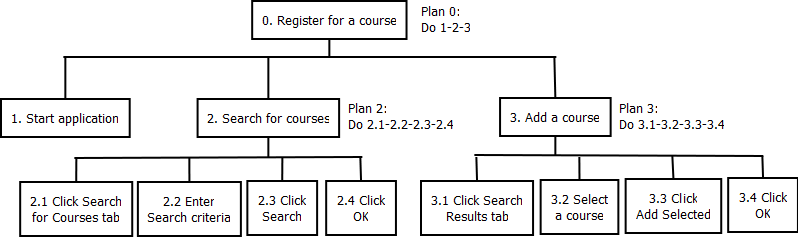
\includegraphics[width=130mm]{05/images/hta}
\end{figure}

\paragraph{CTT (Concurrent Task Tree)} Podobný strom jako HTA, ale s operátory a symboly. Úloha přihlášení: vyplním uživatelské jméno a zároveň heslo, pak je mi umožněho se připojit.

\begin{figure}[h]
\centering
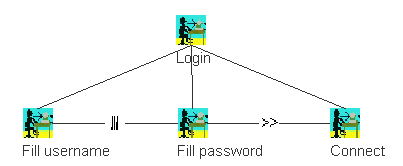
\includegraphics[width=100mm]{05/images/ctt}
\end{figure}
\vspace{-15px}
\begin{itemize}[itemsep=0px]
\item Enabling T1 $>>$ T2
\item Disabling T1 [> T2
\item Interruption T1 |> T2
\item Choice T1 [] T2
\item Iteration T1* nebor T1$_{n}$
\item Concurrency T1 ||| T2
\item Optionality [T]
\end{itemize}


\paragraph{Storyboard} Série snímků a skečů (\uv{komiks} popisující nějakou úlohu).

\paragraph{Scénáře} Jednoduché výpravné příběhy průběhu úkolu

\textit{\uv{Uživatel napíše všechny účastníky akce, vyplní místo a datum konání. Systém poté zkontroluje zda je vše vyplněno v pořádku a vytvoří událost.}}.

\paragraph{Případy užití} Popis interakce člověka se systémem..

\paragraph{Keystroke-Level Model (KLM)}
Cílem je vypočítat čas potřebný pro provedení úlohy
Operátory:
\begin{itemize}[itemsep=0px]
\item stisk klávesy (\textbf{K}eystroke) - určený rychlostí psaní
\item ukázat na cíl na displeji (\textbf{P}ointing) - určeno pomocí Fitt's Law
\item položit ruku na vstupní zařízení (\textbf{H}oming) - odhad měřením
\item mentální příprava akce (\textbf{M}ental preparation) - odhad měřením, heuristika pro předřazení
\item čas reakce systému (\textbf{R}eaction)
\end{itemize}
Jsou časové odhady (tabulkové) pro každý operátor. Předpokládá provádění úloh bez chyby, předpovídá jen efektivitu, ignoruje paralelní zpracování, prokládání úloh, mentální zátěž, plánování a řešení úlohy (\uv{přemýšlecí} čas, uvažovány jsou jen holé akce)


\paragraph{Goals, Operators, Methods, Selection Rules (GOMS)}
Nejznámější používaná metoda. Složky:
\begin{itemize}[itemsep=0px]
\item \textbf{Goals} - cíle z hlediska úmyslů koncového uživatele
\item  \textbf{Operators} - elementární perceptuální, kognitivní a motorické akce s fixním časem
bez ohledu na kontext
\item \textbf{Methods} - posloupnost operátorů a podcílů
\item \textbf{Selection rules} - if-then pravidla určující, kterou metodu použít
\end{itemize}

Předpokládá provádění úloh bez chyby, úlohy musí mít přesně definovaný cíl, nemodeluje proces řešení problému, chování uživatele

\paragraph{Dialog modeling}
Z HTA máme představu o posloupnosti kroků, potřebujeme popsat, jak při provádění kroků spolu budou komunikovat uživatel a počítač - jak bude probíhat dialog
\begin{itemize}[itemsep=0px]
\item textové (gramatiky, produkční pravidla, událostní algebry)
\item diagramy - (STN, PN, flowcharts, JSD)
\end{itemize}

\paragraph{State Transition Networks (STN)}
Varianta konečných automatů, konečný počet stavů a přechodů mezi nimi, automat se nachází v pravě jednom stavu (stavy jsou disjunktní). Reakcí na každý uživatelský vstup je přechod z daného stavu do nového stavu. Stav má přiřazenou akci, musí být odlišitelný od jiných stavů, charakterizován vstupy, které k němu vedou. Přechod mezi stavy může být vázán podmínkou, lze k nim přiřazovat popis akcí.
\begin{itemize}[itemsep=0px]
\item[$+$] model UI, se kterým lze experimentovat
\item[$+$] možnost automatického nebo poloautomatického vytváření UI
\item[$+$] kontrola vlastností (úplnost, reversibilita, dostupnost, nebezpečné stavy - ukončení bez uložení)
\item[$-$] některá zařízení mohou mít velká množství stavů
\end{itemize}

\begin{figure}[h]
\centering
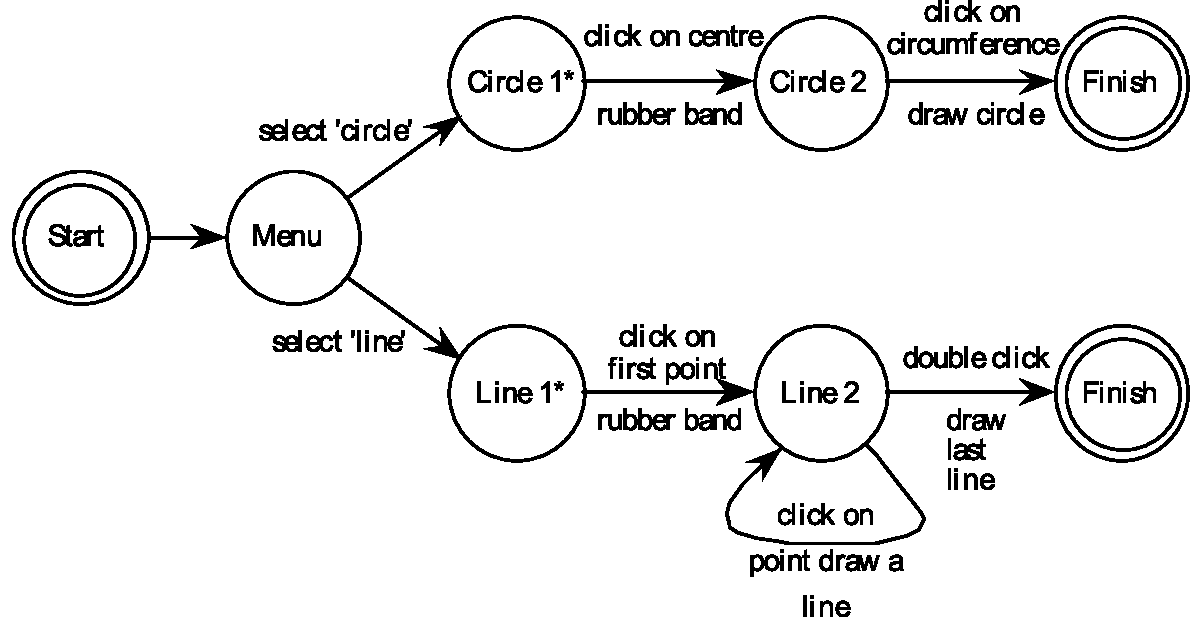
\includegraphics[width=130mm]{05/images/stn}
\end{figure}

\textbf{hierarchické STN} - varianta pro popis složitých dialogů, obsahuje sub-dialogy (vnořené další sítě).

\paragraph{Petriho sítě (PN)} Oproti STN mají synchronizaci - pokračování při splněné podmínce